\documentclass[aspectratio=169,12pt]{beamer}
\usepackage{pgfpages}
\mode<presentation> {
  \usetheme{metropolis}
}

\usepackage{lipsum}
% \usepackage[colorgrid,gridunit=pt,texcoord]{eso-pic}
\usepackage[absolute,overlay]{textpos}
\usepackage{pythonhighlight}
\usepackage[absolute,overlay]{textpos}
\usepackage{url}
\usepackage{caption}
\usepackage{hyperref}
\usepackage[
    type={CC},
    modifier={by},
    version={3.0},
]{doclicense}
\usepackage[whole]{bxcjkjatype}

\setbeamertemplate{note page}{\pagecolor{yellow!5}\vfill\insertnote\vfill}
\setbeameroption{show notes on second screen=right}

\lstset{
language = Python,
breaklines = true,
basicstyle=\fontsize{7}{7}\selectfont\ttfamily,
commentstyle = {\itshape \color[cmyk]{1,0.4,1,0}},
keywordstyle = {\bfseries \color[cmyk]{0,1,0,0}},
stringstyle = {\ttfamily \color[rgb]{1,0,0}},
frame = single,
}
\hypersetup{
colorlinks=true,
}

\title{Visualize 3D scientific data in a Pythonic way like matplotlib}

\begin{document}
\author{Tetsuo Koyama}
\institute{PyVista developer team}

\frame{\titlepage}
\note{
Hi my name is Tetsuo Koyama. Today I will talk about the title "Visualize 3D scientific data in a Pythonic way like matplotlib".

こんにちは、Tetsuo Koyamaです。本日は、「Pythonicに3次元データを可視化しよう」というタイトルでお話します。
}

\begin{frame}[fragile]
\begin{textblock*}{350pt}(50pt, 20pt)
\begin{block}{Who am I?}
\note{
Let me introduce myself first.

まずは自己紹介をさせてください。

}
\end{block}
\end{textblock*}
\begin{textblock*}{350pt}(50pt, 70pt)

\includegraphics[width=0.25\linewidth]{tkoyama010.png}
\end{textblock*}
\begin{textblock*}{350pt}(50pt, 170pt)

\includegraphics[width=0.05\linewidth]{twitter-5662063_1280.png}
\end{textblock*}
\begin{textblock*}{350pt}(70pt, 175pt)
\href{https://twitter.com/tkoyama010}{@tkoyama010}
\end{textblock*}
\begin{textblock*}{350pt}(50pt, 200pt)
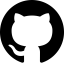
\includegraphics[width=0.05\linewidth]{github.png}
\end{textblock*}
\begin{textblock*}{350pt}(70pt, 205pt)
\href{https://github.com/tkoyama010}{@tkoyama010}
\end{textblock*}
\begin{textblock*}{350pt}(150pt, 25pt)
\begin{itemize}
\item Scientific simulation software engineer.
\note{
I am mechanical simulation software engineer in my careers.

私は科学シミュレーションのソフトウェアエンジニアとして働いています。

}
\item Stuff of Scipy Japan 2020.
\note{
And I was a staff of Scipy Japan 2020.

そして、Scipy Japan 2020のスタッフを務めました。

}
\item PyVista developer team member.
\note{
Also I am a member of PyVista developer team.

また、PyVista開発チームのメンバーでもあります。

}
\item Science, Python, Anime, and Manga.
\note{
I love Science, Python, Anime and Manga.

科学、Python、アニメ、マンガが大好きです。

}
\end{itemize}
\end{textblock*}
\begin{textblock*}{350pt}(200pt, 120pt)
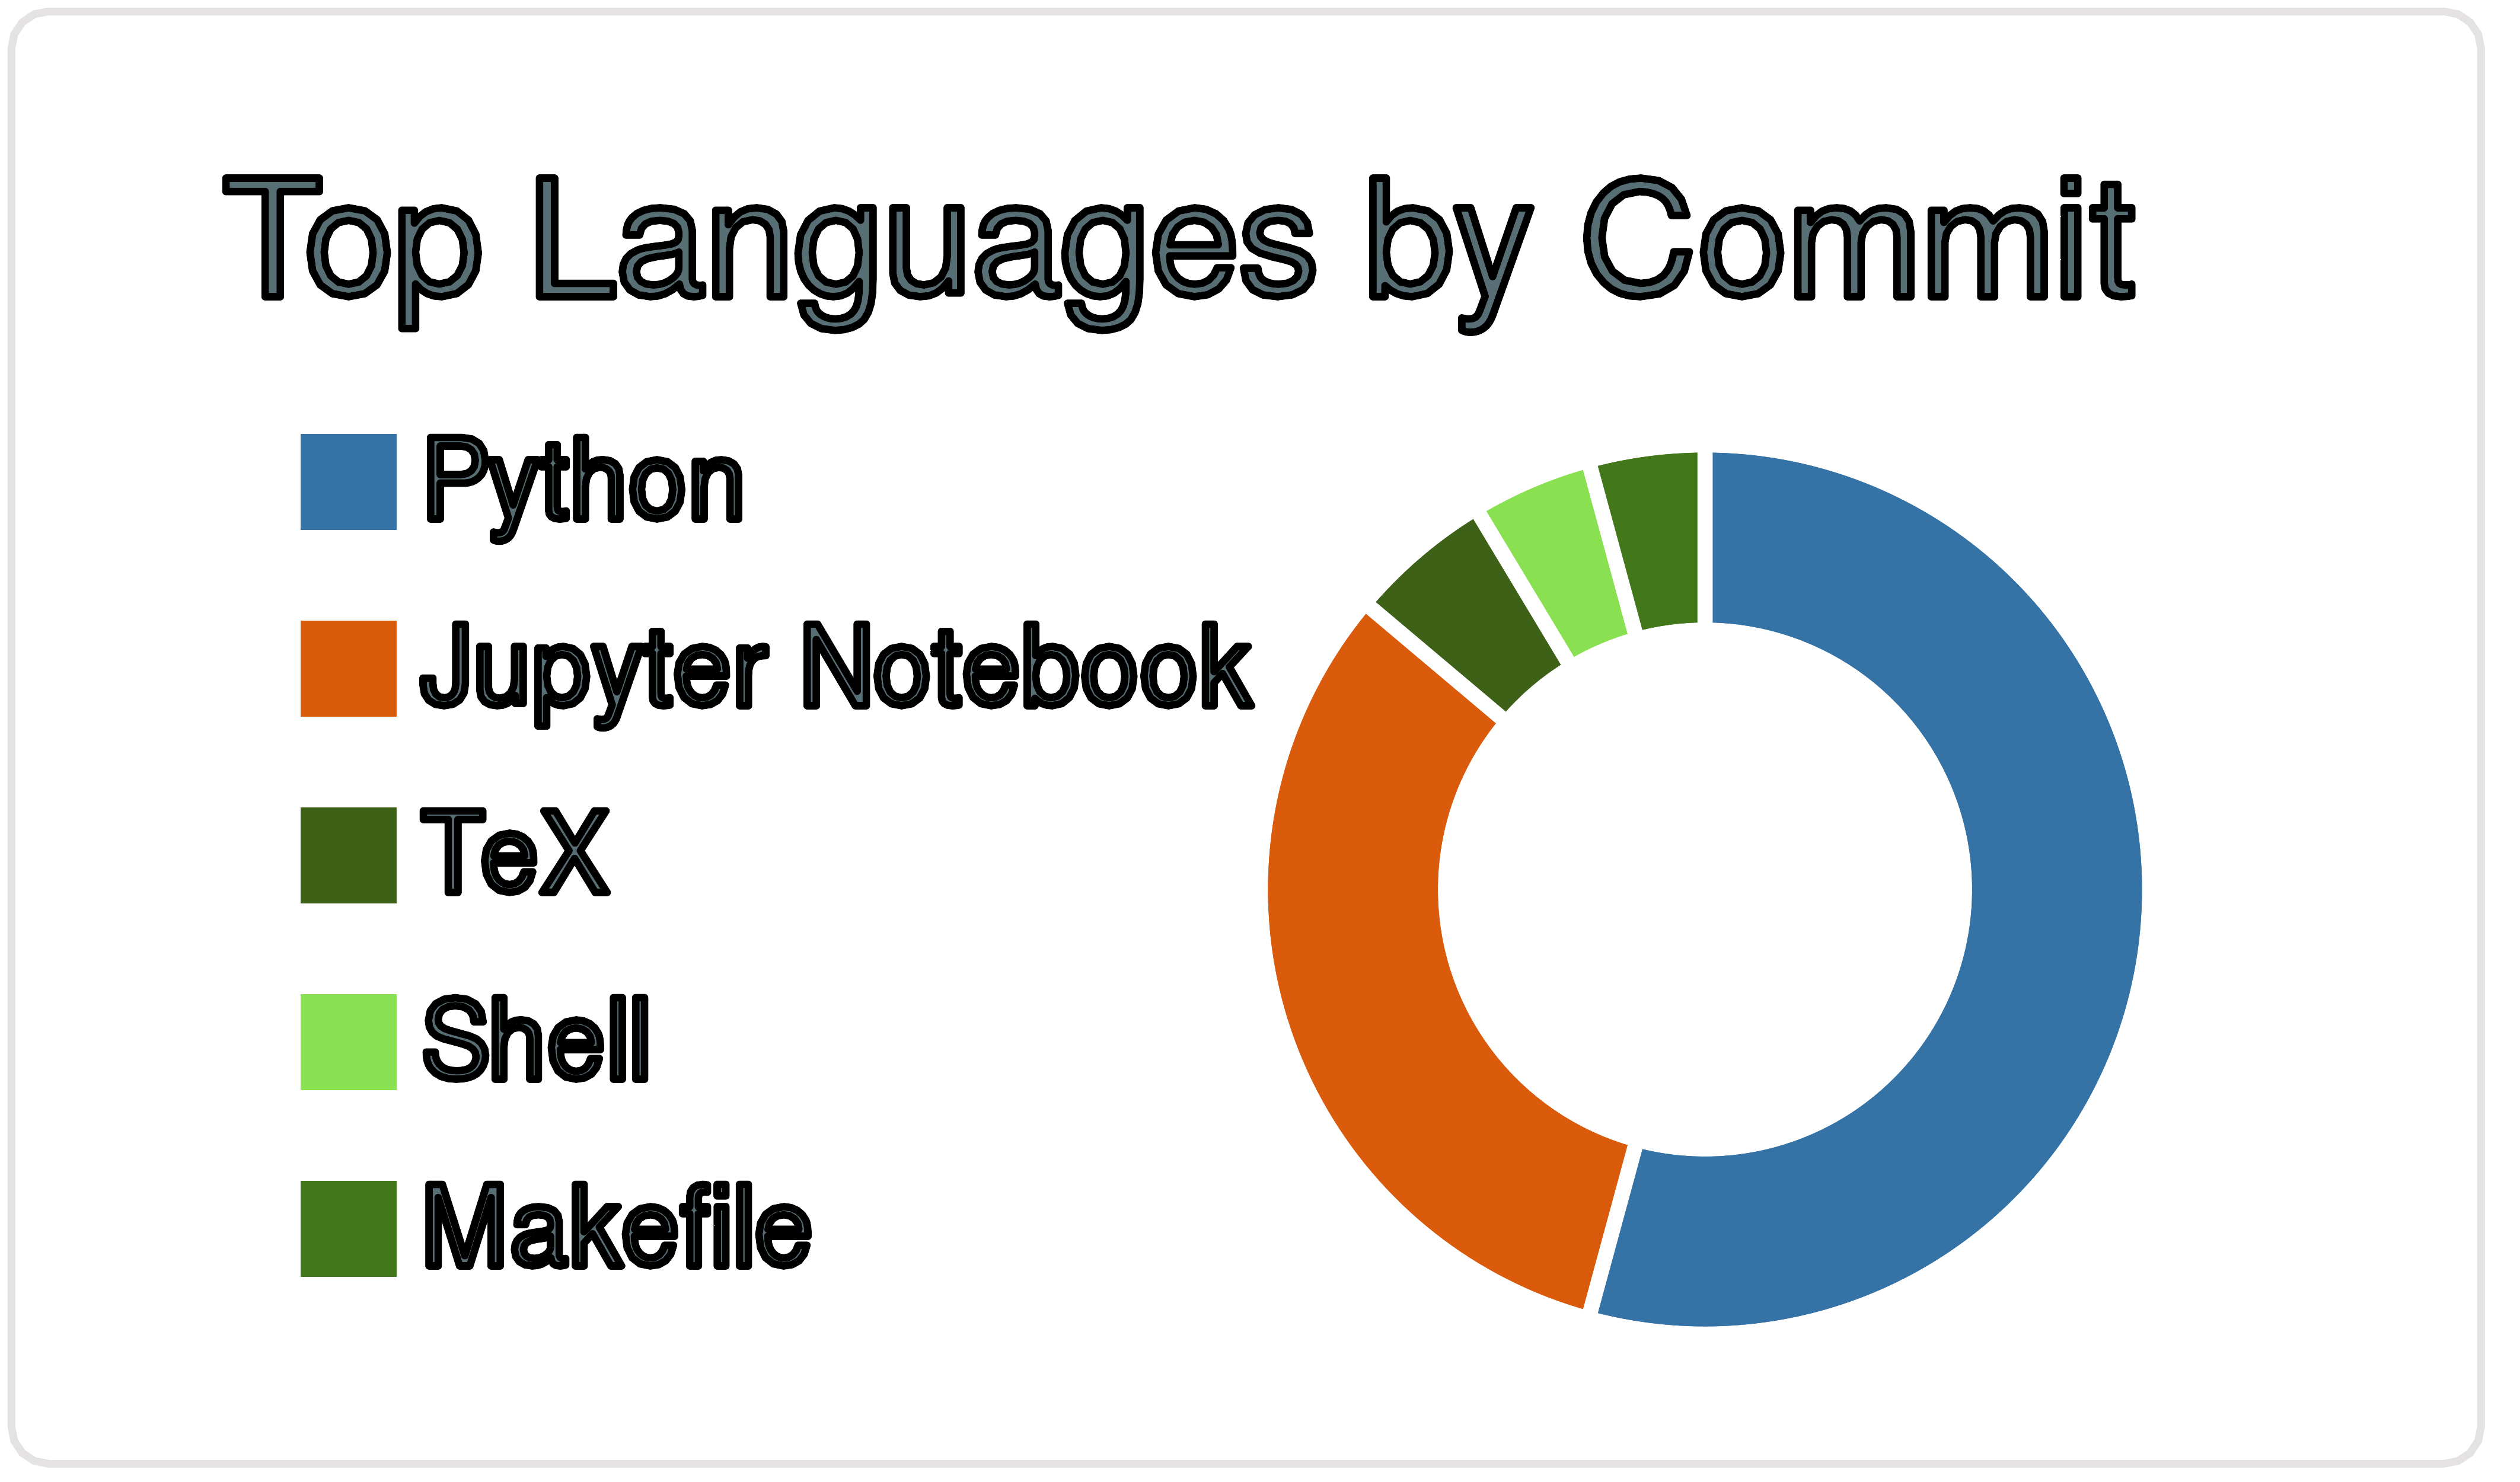
\includegraphics[width=0.50\linewidth]{2-most-commit-language.png}
\end{textblock*}
\note{
My Twitter and Github accounts are \href{https://twitter.com/tkoyama010}{@tkoyama010}.

私のTwitterとGithubのアカウントは\href{https://twitter.com/tkoyama010}{@tkoyama010}です。

}
\note{
Please follow me if you like this presentation.

このプレゼンテーションを気に入っていただけたら、ぜひフォローしてください。
}
\end{frame}

\begin{frame}[fragile]
\begin{textblock*}{800pt}(50pt, 20pt)
\begin{block}{What we want to do is using VTK like matplotlib in PyVista.}
\note{
Do you want to visualize 3D scientific data in a Pythonic way like matplotlib?

matplotlibのようにPythonicな方法で3D科学データを視覚化したいと思いませんか?

}
\note{
If you want, this slides is for you.

望むなら、このスライドはあなたのためのものです。

}
\note{
This slides is the introduction of \href{https://pypi.org/project/pyvista/}{PyVista}.

このスライドは、\href{https://pypi.org/project/pyvista/}{PyVista}の紹介です。

}
\note{
It is

このライブラリには3つの特徴があります。

}
\begin{itemize}
\item "VTK for humans"\: a high-level API to the Visualization Toolkit (VTK)
\note[item]{
"VTK for humans"\: a high-level API to the Visualization Toolkit (VTK)

1つ目は"人間のためのVTK"\: 可視化ツールキット(VTK)の高レベルAPIです。

}
\item 3D plotting made simple and built for large/complex data geometries
\note[item]{
3D plotting made simple and built for large/complex data geometries

2つ目は大規模/複雑なデータ形状に対応した、シンプルな3Dプロッティング機能です。

}
\item mesh data structures and filtering methods for spatial datasets
\note[item]{
mesh data structures and filtering methods for spatial datasets

3つ目はメッシュデータ構造と空間データのフィルタリングメソッドです。

}
\end{itemize}
\end{block}
\end{textblock*}
\begin{textblock*}{800pt}(50pt, 100pt)
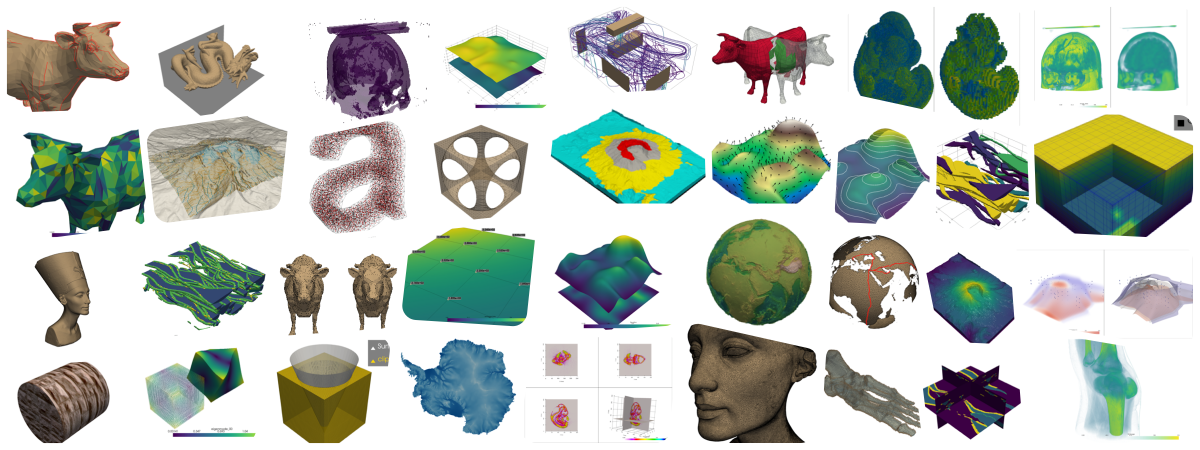
\includegraphics[width=0.50\linewidth]{pyvista_banner_small.png}
\end{textblock*}
\end{frame}

\begin{frame}[fragile]
\begin{textblock*}{350pt}(50pt, 10pt)
\begin{block}{Hello World!}
\note{
In Code Listing \ref{hello_world_code}, we demonstrate the "Hello World!" of \href{https://pypi.org/project/pyvista/}{PyVista}.

コードリスト\ref{hello_world_code}では、\href{https://pypi.org/project/pyvista/}{PyVista}の "Hello World!" を実演しています。

}
\note{
Basic step of \href{https://pypi.org/project/pyvista/}{PyVista} script is the following.

\href{https://pypi.org/project/pyvista/}{PyVista} スクリプトの基本ステップは以下の通りです。

}
\note{
First, import \href{https://pypi.org/project/pyvista/}{PyVista}.

まず、 \href{https://pypi.org/project/pyvista/}{PyVista} をインポートします。

}
\note{
Then generate \href{https://dev.pyvista.org/getting-started/what-is-a-mesh.html}{mesh} and add it to

次に \href{https://dev.pyvista.org/getting-started/what-is-a-mesh.html}{mesh} を生成して、それを

}
\note{
Plotter object using add mesh method.

add meshメソッドを使用してPlotterオブジェクトに追加します。

}
\lstinputlisting[caption=Hello World!, label=hello_world_code, firstline=1, lastline=100]{hello_world.py}
\end{block}
\end{textblock*}
\end{frame}

\begin{frame}[fragile]
\begin{textblock*}{350pt}(50pt, 10pt)
\begin{block}{Hello World!}
\end{block}
\end{textblock*}
\begin{textblock*}{350pt}(50pt, 50pt)
\begin{block}{}
\begin{figure}
\includegraphics[width=1.0\linewidth]{hello_world.png}
\caption{Hello World!\label{HelloWorldFigure}}
\end{figure}
\note{
And finally, we can check the render view (Figure \ref{HelloWorldFigure}) of PyVista using show method.

最後に、showメソッドを使って、PyVistaのレンダリングビュー(図 \ref{HelloWorldFigure})を確認します。
}
\end{block}
\end{textblock*}
\end{frame}

\begin{frame}[fragile]
\begin{textblock*}{350pt}(50pt, 10pt)
\begin{block}{General filters to any data type}

\lstinputlisting[caption=Shrink Mesh, label=ShrinkFilterCode, firstline=4, lastline=5]{shrunk_mesh.py}
\begin{figure}
\includegraphics[width=1.0\linewidth]{shrink.png}
\caption{Shrink filter\label{ShrinkFilterFigure}}
\end{figure}
\note{
\href{https://dev.pyvista.org/core/filters.html}{PyVista classes} hold methods to apply general filters to any data type.

\href{https://dev.pyvista.org/core/filters.html}{PyVistaのクラス} は、任意のデータ型に一般的なフィルタを適用するメソッドを保持しています。

A user can easily apply common filters in an intuitive manner.

ユーザーは直感的なメソッドで簡単に共通のフィルターを適用することができます。

For example, Code Listing \ref{ShrinkFilterCode} shrink the individual faces of a mesh using shrink method (Figure \ref{ShrinkFilterFigure}).

例えば、コードリスト \ref{ShrinkFilterCode} では、シュリンクメソッドを使ってメッシュの各面を縮小しています(図 \ref{ShrinkFilterFigure})。

}
\end{block}
\end{textblock*}
\end{frame}

% \begin{frame}[fragile]
% \begin{textblock*}{350pt}(50pt, 10pt)
% \begin{block}{Rotation about the x axis}
% \note{
% We can of course rotate the mesh about the axes.
%
% もちろん、軸を中心にメッシュを回転させることもできます。
%
% Let's rotate a mesh about its axes.
%
% メッシュを軸周りに回転させてみましょう。
%
% In this model, the x axis is from the left to right; the y axis is from bottom to top; and the z axis emerges from the image.
%
% このモデルでは、x軸は左から右へ、y軸は下から上へ、z軸は画面から垂直になっています。
%
% The camera location is the same in two images.
%
% カメラの位置は2つの画像で同じです。
%
% Rotate the mesh about the x axis every 60 degrees and we can plot it.
%
% このメッシュをx軸を中心に60度ごとに回転させてプロットできます。
%
% Of cource, we can plot also about other axis.
%
% もちろん、他の軸についてもプロットできます。
%
% }
% \end{block}
% \lstinputlisting[caption=X-Axis Rotation, firstline=66, lastline=69]{rotate.py}
% \begin{figure}
% \includegraphics[width=1.0\linewidth]{rotate_x.png}
% \caption{X-Axis Rotation}
% \end{figure}
% \end{textblock*}
% \end{frame}
%
% \begin{frame}[fragile]
% \begin{textblock*}{350pt}(50pt, 10pt)
% \begin{block}{Rotation about the y axis}
% \note{
% Plot the mesh rotated about the y axis every 60 degrees.
%
% メッシュを60度ごとにY軸を中心に回転させてプロットします。
%
% Add the axes actor to the Plotter and set the axes origin to the point of rotation.
%
% プロッターに軸アクターを追加し、軸の原点を回転点に設定しています。
%
% }
% \end{block}
% \lstinputlisting[caption=Y-Axis Rotation, firstline=66, lastline=69]{rotate.py}
% \begin{figure}
% \includegraphics[width=1.0\linewidth]{rotate_y.png}
% \caption{Y-Axis Rotation}
% \end{figure}
% \end{textblock*}
% \end{frame}
%
% \begin{frame}[fragile]
% \begin{textblock*}{350pt}(50pt, 10pt)
% \begin{block}{Rotation about the z axis}
% \note{
% Plot the mesh rotated about the z axis every 60 degrees.
%
% メッシュを60度ごとにz軸を中心に回転させてプロットします。
%
% Add the axes actor to the Plotter and set the axes origin to the point of rotation.
%
% プロッターに軸アクターを追加し、軸の原点を回転点に設定しています。
%
% }
% \end{block}
% \lstinputlisting[caption=Z-Axis Rotation, firstline=66, lastline=69]{rotate.py}
% \begin{figure}
% \includegraphics[width=1.0\linewidth]{rotate_z.png}
% \caption{Z-Axis Rotation}
% \end{figure}
% \end{textblock*}
% \end{frame}
%
% \begin{frame}[fragile]
% \begin{textblock*}{350pt}(50pt, 10pt)
% \begin{block}{Rotation about a custom vector}
% \note{
% Plot the mesh rotated about a custom vector every 60 degrees.
%
% メッシュを60度ごとのカスタムベクトルで回転させてプロットします。
%
% Add the axes actor to the Plotter and set axes origin to the point of rotation.
%
% プロッターに軸アクターを追加し、軸の原点を回転点に設定しています。
%
% }
% \end{block}
% \lstinputlisting[caption=Custom Rotation, firstline=66, lastline=69]{rotate.py}
% \begin{figure}
% \includegraphics[width=1.0\linewidth]{rotate_custom.png}
% \caption{Custom Rotation}
% \end{figure}
% \end{textblock*}
% \end{frame}
%
\begin{frame}[fragile]
\begin{textblock*}{350pt}(50pt, 10pt)
\begin{block}{General filters to any data type}
\lstinputlisting[caption=Extrude Rotate, label=ExtrudeRotateCode, firstline=7, lastline=9]{extrude_rotate.py}
\begin{figure}
\includegraphics[width=1.0\linewidth]{extrude_rotate.png}
\caption{Extrude Rotation\label{ExtrudeRotateFigure}}
\end{figure}
\note{
Code Listing \ref{ExtrudeRotateCode}  creating "skirt" from line
using extrude rotate method (Figure \ref{ExtrudeRotateFigure}).

コードリスト \ref{ExtrudeRotateCode} では、押出し回転メソッドを使って直線から "skirt" を
作成しています (図\ref{ExtrudeRotateFigure}) 。
}
\end{block}
\end{textblock*}
\end{frame}

\begin{frame}[fragile]
\begin{textblock*}{350pt}(50pt, 10pt)
\begin{block}{Load and plot from a files}
\lstinputlisting[caption=Load meshs from the many supported file formats, label=ReadFileCode, firstline=5, lastline=8]{read_file.py}
\begin{figure}
\includegraphics[width=0.6\linewidth]{read_file.png}
\caption{Meshs from the many supported file formats\label{ReadFileFigure}}
\end{figure}
\note{
Loading a \href{https://dev.pyvista.org/getting-started/what-is-a-mesh.html}{mesh} is trivial - if your data is in one of the many supported file formats,
simply use \href{https://dev.pyvista.org/utilities/utilities.html}{pyvista.read()}
to load your spatially referenced dataset into a \href{https://pypi.org/project/pyvista/}{PyVista} \href{https://dev.pyvista.org/getting-started/what-is-a-mesh.html}{mesh} object
(Code Listing \ref{ReadFileCode}, Figure \ref{ReadFileFigure}).

\href{https://dev.pyvista.org/getting-started/what-is-a-mesh.html}{mesh} のロードは簡単です。
データがサポートされている多くのファイルフォーマットのいずれかである場合、
単に \href{https://dev.pyvista.org/utilities/utilities.html}{pyvista.read()} を使用して空間的に参照されたデータセットを
\href{https://pypi.org/project/pyvista/}{PyVista} \href{https://dev.pyvista.org/getting-started/what-is-a-mesh.html}{mesh} オブジェクトにロードします
(コードリスト\ref{ReadFileCode}、図\ref{ReadFileFigure})。

}
\end{block}
\end{textblock*}
\end{frame}

\begin{frame}[fragile]
\begin{textblock*}{350pt}(50pt, 10pt)
\begin{block}{Load and plot from a files}
\lstinputlisting[caption=Save meshs to the many supported file formats, label=SaveFileCode, firstline=26, lastline=29]{read_file.py}
\begin{figure}
\includegraphics[width=0.6\linewidth]{read_file.png}
\caption{Meshs from the many supported file formats\label{ReadFileFigure}}
\end{figure}
\note{
Also note that we can export any \href{https://pypi.org/project/pyvista/}{PyVista} mesh to any file format supported by \href{https://pypi.org/project/meshio/}{meshio}.

また、任意の \href{https://pypi.org/project/pyvista/}{PyVista} メッシュを \href{https://pypi.org/project/meshio/}{meshio} でサポートされている任意のファイルフォーマットにエクスポートできることにも注意してください。

To save a \href{https://pypi.org/project/pyvista/}{PyVista} mesh using meshio, use \href{https://dev.pyvista.org/utilities/utilities.html}{pyvista.save\_meshio()}(Code Listing \ref{SaveFileCode}):

meshioを使って \href{https://pypi.org/project/pyvista/}{PyVista} のメッシュを保存するには、 \href{https://dev.pyvista.org/utilities/utilities.html}{pyvista.save\_meshio()} を使います(コードリスト \ref{SaveFileCode} )。

}
\end{block}
\end{textblock*}
\end{frame}

\begin{frame}[fragile]
\begin{textblock*}{350pt}(50pt, 10pt)
\begin{block}{Extracting and Contouring}
\lstinputlisting[caption=Extracted by scalar, label=WarpScalarCode, firstline=9, lastline=9]{contour.py}
\begin{figure}
\includegraphics[width=0.5\linewidth]{contour.png}
\caption{Contouring\label{WarpScalarFigure}}
\end{figure}
\note{
Attributes are data values that live on either the nodes or cells of a mesh.

Attributeとは、メッシュのノードまたはセル上に存在するデータ値のことです。

In \href{https://pypi.org/project/pyvista/}{PyVista}, we work with both point data and cell data and allow easy access to data dictionaries to hold arrays for attributes that live either on all nodes or on all cells of a mesh.

\href{https://pypi.org/project/pyvista/}{PyVista} では、ポイントデータとセルデータの両方を扱い、メッシュのすべてのノードまたはすべてのセルに存在する属性の配列を保持するデータ辞書に簡単にアクセスできるようにしています。

Meshes can have a scalar field extracted using \href{https://dev.pyvista.org/core/filters.html}{warp\_by\_scalar()} method (Code List \ref{WarpScalarCode}, Figure \ref{WarpScalarFigure}).

\href{https://dev.pyvista.org/core/filters.html}{warp\_by\_scalar()} メソッドでメッシュからスカラーフィールドを抽出することができます(コードリスト \ref{WarpScalarCode} 、図 \ref{WarpScalarFigure} )。

}
\end{block}
\end{textblock*}
\end{frame}

\begin{frame}[fragile]
\begin{textblock*}{350pt}(50pt, 10pt)
\begin{block}{Plot data over circular arc}
\lstinputlisting[caption=Plotting over circular arc, label=PlotOverCircularArcCode, firstline=10, lastline=18]{kitchen.py}
\end{block}
\end{textblock*}
\begin{textblock*}{300pt}(0pt, 110pt)
\begin{block}{}
\note{
It can be plotting the values of a dataset over a circular arc through that dataset using
\href{https://dev.pyvista.org/core/filters.html}{plot\_over\_circular\_arc\_normal}
(Code list \ref{PlotOverCircularArcCode}, Figure \ref{CircularArcToPlotFigure} and \ref{PlotOverCircularArcFigure}).

\href{https://dev.pyvista.org/core/filters.html}{plot\_over\_circular\_arc\_normal}
を使用して、データセットを通る円弧上のデータセットの値をプロットすることができます
(コードリスト\ref{PlotOverCircularArcCode}、図\ref{CircularArcToPlotFigure}および\ref{PlotOverCircularArcFigure})。

}
\begin{figure}
\includegraphics[width=0.5\linewidth]{kitchen.png}
\caption{Circular arc to plot \label{CircularArcToPlotFigure}}
\end{figure}
\end{block}
\end{textblock*}
\begin{textblock*}{350pt}(150pt, 130pt)
\begin{figure}
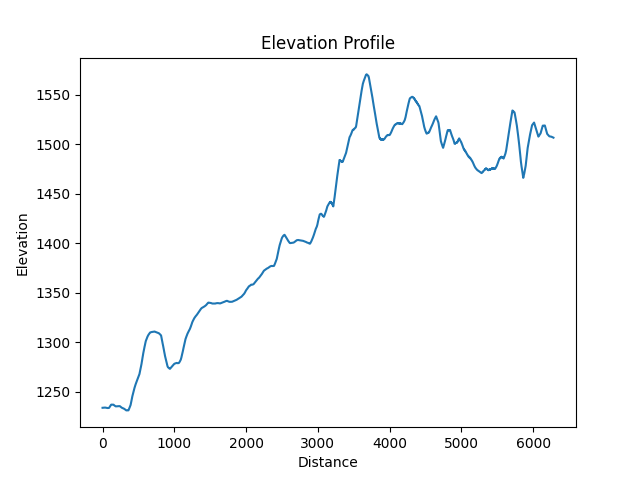
\includegraphics[width=0.3\linewidth]{elevation.png}
\caption{Plot over line \label{PlotOverCircularArcFigure}}
\end{figure}
\end{textblock*}
\end{frame}

\begin{frame}[fragile]
\begin{textblock*}{350pt}(50pt, 10pt)
\begin{block}{Extracting and Contouring}
\lstinputlisting[caption=Extracted by vector, label=WarpVectorCode, firstline=44, lastline=44]{contour.py}
\begin{figure}
\includegraphics[width=1.0\linewidth]{warped_vector.png}
\caption{Warped sphere by vector\label{WarpVectorFigure}}
\end{figure}
\note{
Also can have a vector filed extracted using \href{https://dev.pyvista.org/core/filters.html}{warp\_by\_vector()} method (Code List \ref{WarpVectorCode}, Figure \ref{WarpVectorFigure}).

また、 \href{https://dev.pyvista.org/core/filters.html}{warp\_by\_vector()} メソッドで抽出されたベクターファイルを持つことができます(コードリスト \ref{WarpVectorCode} 、図 \ref{WarpVectorFigure} )。

\href{https://dev.pyvista.org/plotting/plotting.html}{add\_mesh()} method can use a Matplotlib, Colorcet, cmocean, or custom colormap when plotting scalar values(Figure \ref{WarpVectorFigure}).

\href{https://dev.pyvista.org/plotting/plotting.html}{add\_mesh () }メソッドは、スカラー値をプロットするときにMatplotlib、Colorcet、cmocean、またはカスタムカラーマップを使用できます (図\ref{WarpVectorFigure}) 。

}
\end{block}
\end{textblock*}
\end{frame}

\begin{frame}[fragile]
\begin{textblock*}{350pt}(50pt, 10pt)
\begin{block}{Camera class}
\begin{figure}
\includegraphics[width=0.75\linewidth]{frustum_of_camera.png}
\caption{Frustum of camera \label{CameraFrustumFigure}}
\end{figure}
\note{
\href{https://dev.pyvista.org/core/camera.html}{Camera} class is a virtual camera for 3D rendering.

\href{https://dev.pyvista.org/core/camera.html}{Camera}クラスは、3 Dレンダリング用の仮想カメラです。

It provides methods to position and orient the view point and focal point.

視点や焦点の位置や方向を決めるメソッドを提供します。

Convenience methods for moving about the focal point also are provided.

また、焦点を移動するための便利なメソッドも提供されています。

More complex methods allow the manipulation of the computer graphics model including view up vector, clipping planes, and camera perspective (Figure \ref{CameraFrustumFigure}).

より複雑なメソッドでは、ビューアップベクター、クリッピングプレーン、カメラパースペクティブなど、コンピュータグラフィックスモデルを操作することができます(図 \ref{CameraFrustumFigure})。

}
\lstinputlisting[caption=Add Camera to Plotter, label=camera_view, firstline=7, lastline=13]{camera_view.py}
\end{block}
\end{textblock*}
\end{frame}

\begin{frame}[fragile]
\begin{textblock*}{350pt}(50pt, 10pt)
\begin{block}{Camera class}
\lstinputlisting[caption=Create camera frustum, label=CameraFrustumCode, firstline=8, lastline=13]{frustum_of_camera.py}
\begin{figure}
\includegraphics[width=0.75\linewidth]{camera_view.png}
\caption{Camera view}
\end{figure}
\note{
Code Listing \ref{CameraFrustumCode} create a camera and frustum.

コードリスト\ref{CameraFrustumCode}ではカメラと視錐台を作成しています。

Then create a scene of inside frustum adding \href{https://dev.pyvista.org/core/camera.html}{Camera} object to \href{https://dev.pyvista.org/plotting/plotting.html}{Plotter} object
(Code list \ref{CameraFrustumCode} ,Figure \ref{CameraFrustumFigure}).

次に、視錐台内部のシーンを作成して、\href{https://dev.pyvista.org/plotting/plotting.html}{Plotter}オブジェクトに\href{https://dev.pyvista.org/core/camera.html}{Camera}オブジェクトを追加します
(コードリスト\ref{CameraFrustumCode}、図\ref{CameraFrustumFigure})。

}
\end{block}
\end{textblock*}
\end{frame}

\begin{frame}[fragile]
\begin{textblock*}{150pt}(50pt, 10pt)
\begin{block}{Controlling Camera Rotation}
\lstinputlisting[caption=Controlling Camera Rotation, label=CameraRotationCode, firstline=29, lastline=29]{camera_view.py}
\lstinputlisting[firstline=34, lastline=34]{camera_view.py}
\lstinputlisting[firstline=39, lastline=39]{camera_view.py}
\end{block}
\end{textblock*}
\begin{textblock*}{350pt}(150pt, 50pt)
\begin{figure}
\includegraphics[width=0.5\linewidth]{camera_rotation.png}
\caption{Controlling Camera Rotation \label{CameraRotationFigure}}
\end{figure}
\note{
In addition to directly controlling the camera position by setting it via the pyvista
\href{https://dev.pyvista.org/core/camera.html}{Camera.position}
property

さらに、pyvistaの\href{https://dev.pyvista.org/core/camera.html}{Camera.position}
プロパティを使用してカメラ位置を設定することにより、カメラ位置を直接制御することもできます。

You can also directly control the
\href{https://dev.pyvista.org/core/camera.html}{pyvista.Camera.roll},
\href{https://dev.pyvista.org/core/camera.html}{pyvista.Camera.elevation}, and
\href{https://dev.pyvista.org/core/camera.html}{pyvista.Camera.azimuth}
of the camera.
(Code list \ref{CameraRotationCode} ,Figure \ref{CameraRotationFigure}).

カメラの
\href{https://dev.pyvista.org/core/camera.html}{pyvista.Camera.roll},
\href{https://dev.pyvista.org/core/camera.html}{pyvista.Camera.elevation},
および\href{https://dev.pyvista.org/core/camera.html}{pyvista.Camera.azimuth}
を直接制御することもできます。
(コードリスト\ref{CameraRotationCode}、図\ref{CameraRotationFigure})

}
\end{textblock*}
\end{frame}

\begin{frame}[fragile]
\begin{textblock*}{350pt}(50pt, 10pt)
\begin{block}{Acknowlegment}
I would like to thank \href{https://github.com/orgs/pyvista/teams/developers}{PyVista developer team} for developing useful library.
\end{block}
\begin{block}{References}
C. Bane Sullivan and Alexander Kaszynski, (2019). PyVista: 3D plotting and mesh analysis through a streamlined interface for the Visualization Toolkit (VTK). Journal of Open Source Software, 4(37), 1450, \url{https://doi.org/10.21105/joss.01450}
\end{block}
\begin{block}{Contact Information}
If you want to know and discuss pyvista more, join \href{http://github.com/pyvista/pyvista/discussions}{GitHub Discussion}.
\end{block}
\note{
I would like to thank PyVista developer team for developing useful library.

役に立つライブラリを開発してくれたPyVista開発チームに感謝します。

If you want to know and discuss pyvista more, join \href{http://github.com/pyvista/pyvista/discussions}{GitHub Discussion}.

pyvistaについてもっと知りたいなら、\href{http://github.com/pyvista/pyvista/discussions}{GitHub Discussion}に参加してください。

}
\doclicenseThis
\end{textblock*}
\end{frame}

\end{document}

